\chapter{Conclusiones del proyecto}\label{sec:conclusion}
En esta sección se realizará un balance del trabajo realizado indicando a su vez varias mejoras que pueden realizarse en las próximas versiones del producto.

El autor considera el proyecto uno de los más interesantes que ha realizado en la carrera, permitiéndole aplicar varios de los conocimientos adquiridos durante la misma. Los conocimientos aplicados varían enormemente, cubriendo conceptos como \textit{DMA} proporcionados en la asignatura de ``Periféricos e Interfaces'', el uso de ondas visto en la asignatura de ``Transmisión de Datos y Redes de Computadores'' e incluso algunos conceptos matemáticos en el área de matrices. El desarrollo de un juego para la Game Boy Advance también ha permitido un mejor entendimiento de varios de los dispositivos con los que el autor ha trabajado anteriormente, en concreto los microcontroladores Arduino y ESPRESSIF mencionados en la introducción del trabajo. Esto último demuestra la efectividad que tiene el dispositivo en el espacio educativo, tal y como se demostró en~\cite{bib:paper3,bib:paper_1,bib:paper_2}.

Además, el autor considera que actualmente tiene un mejor entendimiento de las tareas a realizar para proyectos futuros que involucren el desarrollo de un videojuego, identificando mejor las tareas que puede realizar y las que no. De las tareas que no se han podido realizar, como el diseño del arte y de la música, el autor considera que con más tiempo este aspecto podría haber sido mejorado dado que acabo siendo un factor limitante durante el desarrollo del juego. Otro aspecto a mejorar, relacionado con el arte del juego, es la poca cantidad de contenido disponible en el producto final ya que los enemigos, personajes y fondos dependían del contenido ``open source'' disponible online. 

A pesar de que el proyecto no ha quedado con los estándares que el autor deseaba, tiene la motivación no solo para seguir desarrollando el proyecto hasta conseguir una versión con la que esté satisfecho, sino para continuar desarrollando juegos para la Game Boy Advance. En sus próximos proyectos, espera combinar los conocimientos ya adquiridos con otros con finalidades más específicas como la comunicación serial que ofrece la consola para comunicarse con otros jugadores.

\section{Trabajo futuro}
A continuación se incluirán las mejoras que el autor considera implementar durante los próximos meses para alcanzar el nivel de calidad deseado. Las mejoras no incluyen las ``remodelaciones'' desde cero que desearía realizar el autor, sino mejoras inmediatas al producto actual.

\begin{itemize}
	\item Mejora del movimiento del jugador, haciendo que los controles sean más fluidos para el jugador.
	\item Mejora en las colisiones del jugador con el mapa. Actualmente las colisiones del jugador con el entorno se realizan de forma aproximada cuando este se mueve a una velocidad no exacta (por ejemplo, al moverse a $1.25$ píxeles por unidad de tiempo). 
	\item Buscar una implementación de la sincronización vertical que permita jugar al juego a 120 Hz en emuladores. El autor no ha investigado al respecto pero cree que es posible y una opción interesante dado que una gran parte de los jugadores utiliza emuladores en dispositivos considerablemente más potentes que la consola original. 
	\item Uso de efectos de sonido para las acciones del personaje principal (por ejemplo, al saltar y atacar). Estos se realizarían con los canales de audio 1, 2, 3 y 4.
	\item Implementación de un sistema de texto que permita el uso de más de un lenguaje. Actualmente el juego solo se encuentra en inglés.
	\item Implementación de un sistema que permita el uso de más de un mago. Esto permitiría añadir más variantes al juego (actualmente solo hay 2). El prototipo que el autor tenía en mente, sería uno similar al ofrecido por otros juegos con varias opciones a seleccionar. El jugador presionaría el botón ``L'' o ``R'', acción que abriría un menú, y con el pad direccional seleccionaría la variante a utilizar. Una imagen mostrando el prototipo se puede observar en la Figura~\ref{fig:menu_proto}.

	\begin{figure}[h]
		\centering
		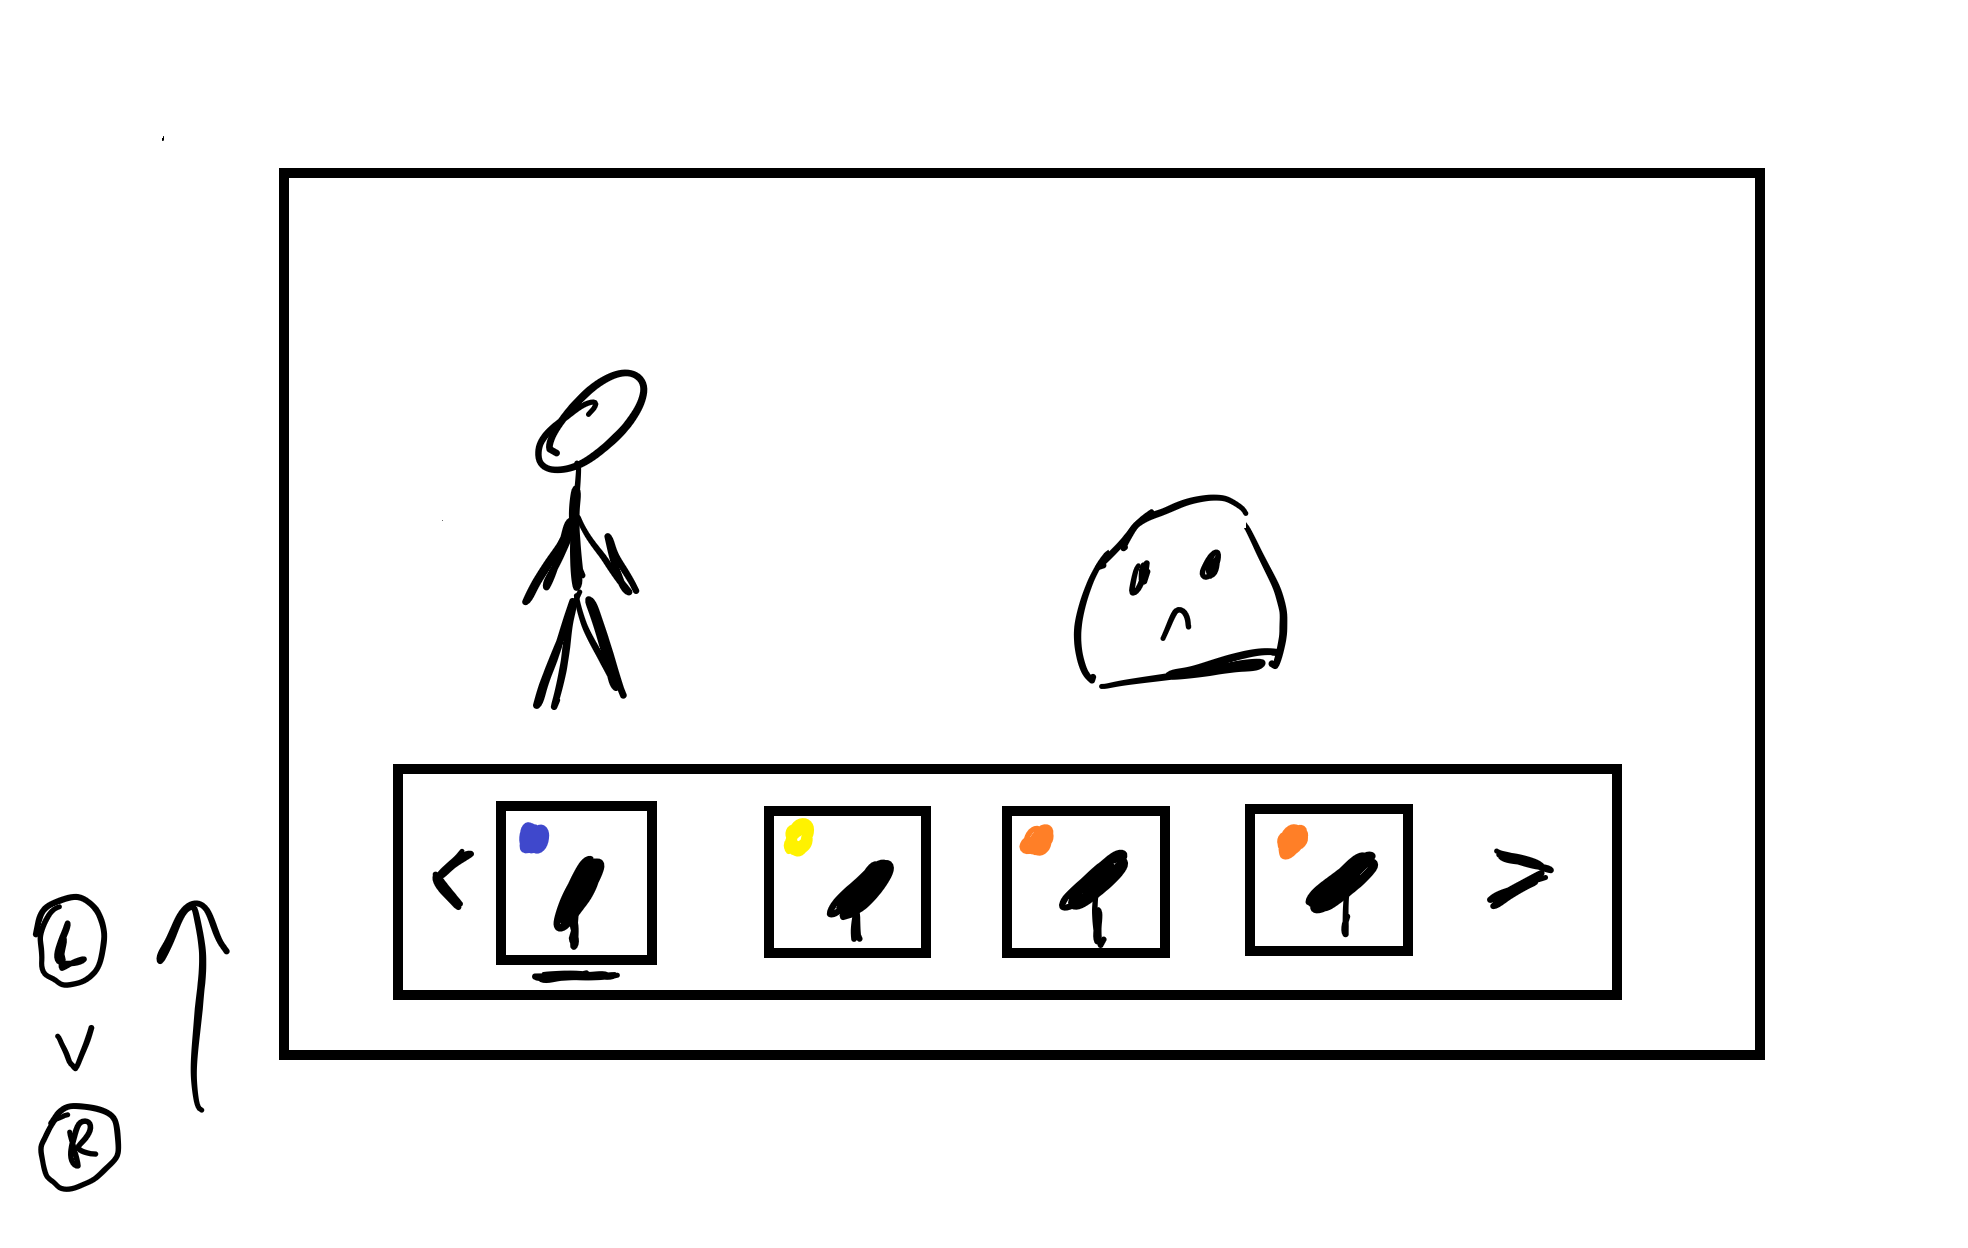
\includegraphics[width=.5\textwidth]{capitulos/capitulo7/proto.png}
		\caption{Prototipo del nuevo sistema de selección.}\label{fig:menu_proto}
	\end{figure}
	\FloatBarrier{}

	\item Implementación de las secciones más costosas en ensamblador. El autor tiene pensado implementar las funciones encargadas de gestionar las colisiones de los enemigos y personaje principal.
\end{itemize}
